% Copyright 2020 by Junwei Wang <i.junwei.wang@gmail.com>
%
% This file may be distributed and/or modified under the
% conditions of the LaTeX Project Public License, either version 1.3c
% of this license or (at your option) any later version.
% The latest version of this license is in
%   http://www.latex-project.org/lppl.txt

% \documentclass[aspectratio=169,compress]{beamer}
\documentclass[aspectratio=169,compress]{beamer}

\usepackage[english]{babel}
\usepackage{metalogo}
\usepackage{listings}
\usepackage{fontspec}
\usepackage{tikz}

% \usetheme{Nord}
\usetheme[style=light]{Nord}


%\usepackage[spanish, es-tabla]{babel}
\usepackage[utf8]{inputenc}
\usepackage{hyperref}




\setmainfont{Yanone Kaffeesatz}
%\setsansfont{Andika New Basic}
\setmonofont{DejaVu Sans Mono}

\setbeamerfont{frametitle}{parent=structure,size=\Large}

\AtBeginSection[]
{
  \begin{frame}[c,noframenumbering,plain]
    \tableofcontents[sectionstyle=show/hide,subsectionstyle=show/show/hide]
  \end{frame}
}

\AtBeginSubsection[]
{
  \begin{frame}[c,noframenumbering,plain]
    \tableofcontents[sectionstyle=show/hide,subsectionstyle=show/shaded/hide]
  \end{frame}
}

\title{Arquitecturas y Organización de Computadoras I}
\subtitle{2: Arquitectura MIPS}
\author{Rafael Ignacio Zurita}
\institute{Depto. Ingeniería de Computadoras}
\date{\today}

\begin{document} 
\begin{frame}[plain,noframenumbering]
\bigskip
  \maketitle
\end{frame}

% video
% mostrar varias computadoritas
% mostrar placa con integrados y pcb
% mostrar foto de chip y hablar de los transistores
% mostrar imagen wakerly de transistor CMOS

% imagenes 
% foto de performance
% cuadro python vs C
% foto eras tecnologicas

% historia de ibm
% fotos de computadoras hitos
%     ibm 360 (mainframe), cray1 (supercoputaodra)
%     pdp-11 (creacion de unix) (minicomputadora)
%     4004 primer chip integrado
%     apple II y ibm pc (computadora personal)
%     open mobile komunications (smartphones)
%     iphone smartphone




\section{Arquitectura MIPS}



\subsection{Máquina MIPS general}

\begin{footnotesize}

\begin{frame}
\frametitle{Introducción a MIPS}
\begin{center}
\begin{figure}
% 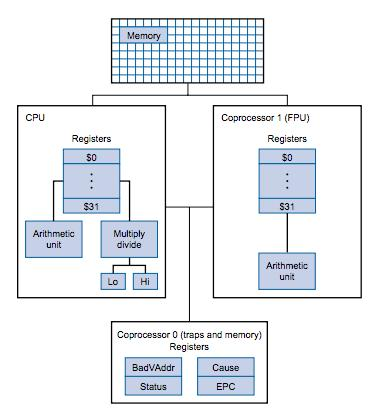
\includegraphics[scale=0.4]{images/organizacion-mips.jpg} 
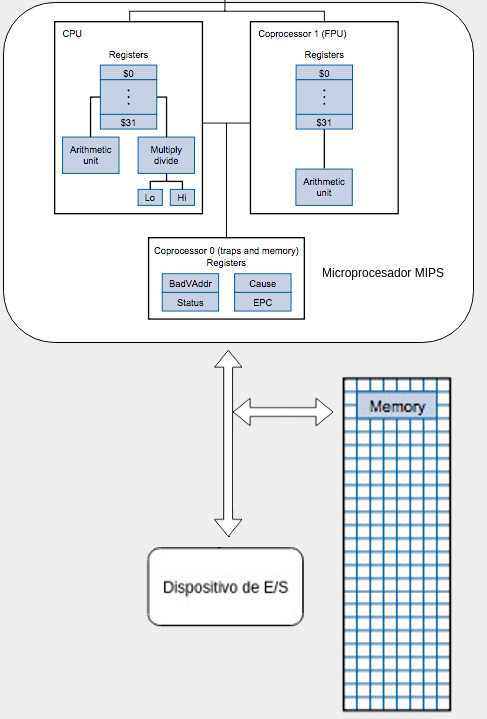
\includegraphics[scale=0.26]{images/mips-arq1.jpg} 
\caption{Diagrama de Bloques de una computadora MIPS}
\label{Diagrama de Bloques de una computadora MIPS}
\end{figure}
\end{center}
\end{frame}


\begin{frame}{MIPS (RISC) vs x86 (CISC)}{Comparativa}
\begin{footnotesize}
 \begin{columns}[onlytextwidth,T]
%      \column{\dimexpr\linewidth-60mm-5mm}

      \column{70mm}
\bigskip
\begin{center}\textbf{Arquitectura MIPS}\end{center}
\begin{itemize}
\item Muchos registros: 32 registros de 32bits (muchos registros)
\item Instrucciones de tamaño fijo (32bits)
\item Pocos formatos de instrucciones
\item Pocos modos de direccionamiento
\item ALU opera con 3 operandos en registros (registro-registro)
\item Conjunto de instrucciones reducido
\item \textbf{Objetivo: Simplicidad para hacer eficiente en hardware el caso mas común}
\end{itemize}

      \column{80mm}

\bigskip
\begin{center}\textbf{Arquitectura AMD64 (x86 de 64bits)}\end{center}
\begin{itemize}
\item Pocos registros: 16 registros de 64bits (la versión 32bits tiene sólo 8 registros)
\item Instrucciones de tamaño variable
\item Muchos formatos de instrucciones
\item Muchos modos de direccionamiento
\item La ALU puede operar con registros, o memoria (registro-memoria)
\item Conjunto de instrucciones complejo
\item \textbf{Objetivo: Compatibilidad con procesadores anteriores de Intel de 16bits y 8bits}
\end{itemize}
    \end{columns}
\end{footnotesize}
\end{frame}



\begin{frame}{MIPS (RISC) vs x86 (CISC)}{Comparativa}

 \begin{columns}[onlytextwidth,T]
%      \column{\dimexpr\linewidth-60mm-5mm}

      \column{90mm}

\begin{center}\textbf{Arquitectura AMD64 (x86 de 64bits)}\end{center}

\begin{itemize}
\begin{scriptsize}
\item Intel y AMD fabrican microarquitecturas AMD64 en chips de alto rendimiento
\item Su performance suele ser mucho mayor a un procesador MIPS
\item Una razón es que MIPS se ha dedicado a procesadores de bajo consumo
\item Otra razón es debido a que los ingenieros de Intel y AMD han incorporado casi todas las mejoras de los últimos 40 años a nivel microarquitectura:
\end{scriptsize}

\begin{itemize}
\begin{tiny}
\item Ejecución especulativa: ejecutar en paralelo instrucciones
\item Renombramiento de registros: Los chips de Intel y AMD incorporan de registros
\item Superscalar y multiples threads
\item Varios cores (CPUs) en el mismo chip
\item Ejecución de cada instrucción máquina a través de microinstrucciones RISC
\item .
\end{tiny}
\end{itemize}

\end{itemize}
      \column{60mm}
\bigskip
\bigskip
\bigskip
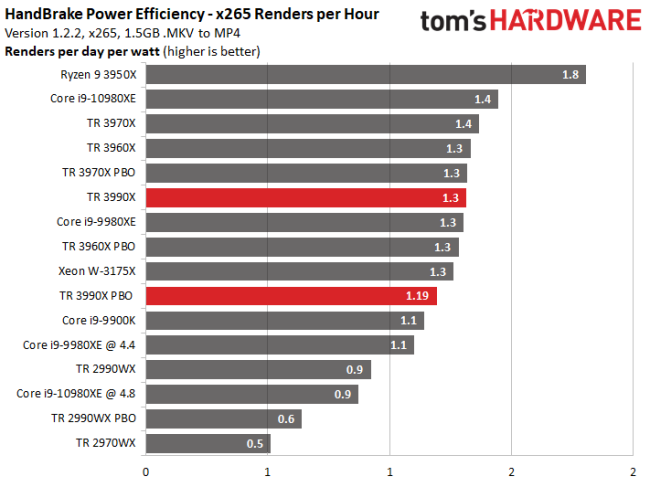
\includegraphics[scale=0.25]{images/intelvsamd.png} 
    \end{columns}
\end{frame}

\subsection{Hardware visible al programador: memoria y registros}

\begin{frame}
\frametitle{Organización de la Memoria principal en MIPS}

 \begin{columns}[onlytextwidth,T]
      \column{\dimexpr\linewidth-60mm-5mm}

\begin{itemize}
	\item La memoria total máxima posible es de \textbf{4GB}.
	\item $2^{32}$ La memoria es \textbf{byte direccionable} (cada byte tiene una dirección de memoria 0, 1, 2 ...) 
	\item $2^{30}$ palabras de 4-bytes, con direcciones 0, 4, 8 ... 
	\item Las direcciones de datos con tamaño de palabra (word, float) deben ser múltiplos de 4.
	\item Las direcciones de las medias palabras (half) deben ser múltiplos de 2.
	\item Las direcciones de las dobles palabras (ej. double) deben ser múltiplos de 8.
\end{itemize}
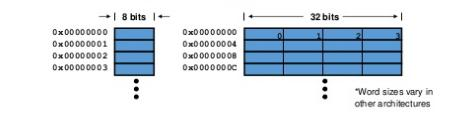
\includegraphics[scale=0.4]{images/memoria-mips.jpg} 

      \column{60mm}
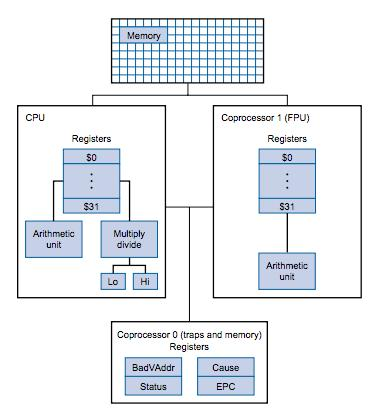
\includegraphics[scale=0.45]{images/organizacion-mips.jpg} 

    \end{columns}
\end{frame}


\begin{frame}
\frametitle{Organización de la Memoria principal en MIPS}

 \begin{columns}[onlytextwidth,T]
      \column{\dimexpr\linewidth-60mm-5mm}

  Un programa en memoria está dividido en segmentos lógicos, para organizar su contenido.
        \begin{itemize}
\bigskip
  \item[Código] En el \textbf{segmento de código} se ubican las instrucciones máquina del programa.
  \item[Datos] En el \textbf{segmento de datos} se ubican las variables globales del programa.
  \item[Pila] En el \textbf{segmento de pila} se ubican las variables locales a una función.

        \end{itemize}

      \column{60mm}
    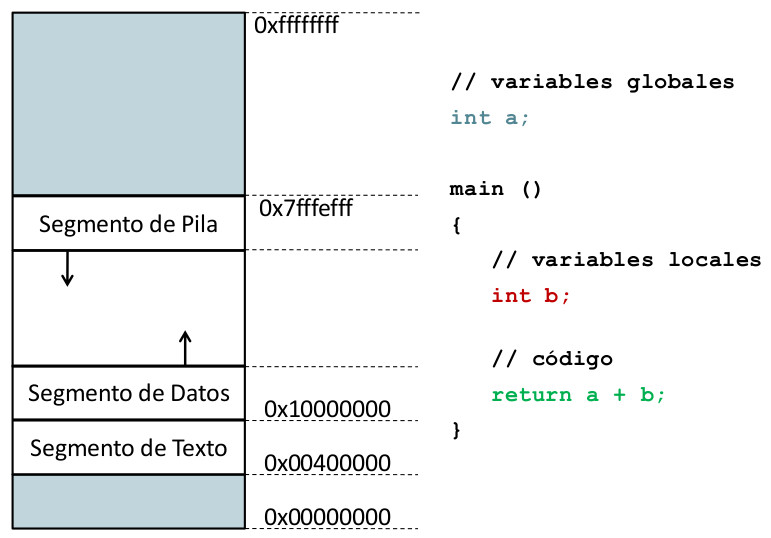
\includegraphics[width=65mm]{images/memoria-programa.jpg}

    \end{columns}


\end{frame}




% INDICE: HISTORIA de procesadores y arquitectura (filmina de arquitectura de david), system 360, zseries, 
% compilacion, ensamblado, codigo maquina
% ejemplo x86 , uso de longitud variable para instruccciones, instrucciongs con dos operandos, pocos registros, infinidad de modos de direccion2miento para cada operacion. En cada version nuevas instrucciones y compatibilidad. Cientos de instrucciones CISC
% Microarquitectura : programada (interprete), en hardware
% grafico inicio de RISC: quitar el interprete, hacer un set sencillo, fijo y de pocos formatos
% limite de energia, nacimiento de arquitecturas avanzadas 
%
% lenguaje ensamblador, figura de compilacion, ejemplo de ensamblador x86, figura de dos arquitecturas x86, system 360, zseries,X , filmina de diferencia entre arquitectura y organizacion, estructura por capas y resumen de los temas a ver en la materia,  memoria, 
% segunda parte: antes de ver lenguaje ensamblador veremos terminologia importante sobre la organizacion  de la memoria
% Representación de datos a nivel de máquina. Direccionamiento de memoria: concepto de palabra, ordenamiento de bytes. Registros.} 
% memori2, direccion, byte, palabra, alineacion, endianess, instrucciones y datos
% directivas MIPS, etc para el practico

\begin{frame}
\frametitle{Registros dentro del procesador}
 \begin{columns}[onlytextwidth,T]
      \column{\dimexpr\linewidth-60mm-5mm}

Registros visibles al usuario.
        \begin{itemize}
\bigskip
  \item[32] Existen 32 registros de propósito general.
  \item[4 bytes] Cada registro tiene el tamaño de la palabra en la arquitectura (32bits/4 bytes).
  \item[Uso] Se los menciona en lenguaje ensamblador colocando un signo \$ (ej. \$t2, o \$5).

        \end{itemize}

Otros registros.
        \begin{itemize}
  \item Existen muchos otros registros, pero son parte de la microarquitectura (buffers, PC, EPC, Cause, etc).
        \end{itemize}
      \column{60mm}
    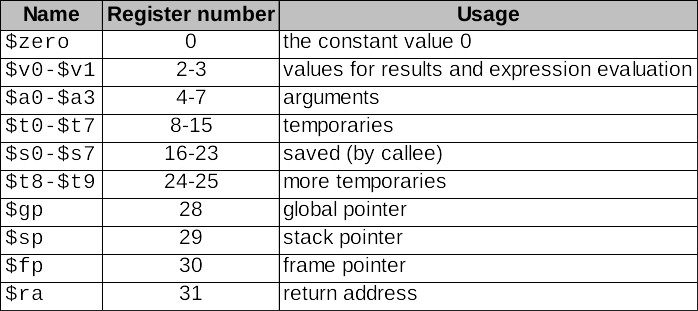
\includegraphics[width=65mm]{images/convencion.jpg}

    \end{columns}


\end{frame}

\subsection{Cuando utilizar lenguaje ensamblador}

\subsection{Conjunto de instrucciones}


\begin{frame}
\frametitle{Tipos de Instrucciones}
\begin{center}\textbf{Tipos Principales de Instrucciones}\end{center}
\begin{itemize}
\item Instrucciones de transferencia de datos (memoria a registro o viceversa)
\begin{itemize}
\item Carga y Almacenamiento
\end{itemize}
\item Aritméticas y Lógicas
\begin{itemize}
\item Enteros
\item Punto Flotante
\end{itemize}
\item Flujo de control
\begin{itemize}
\item Salto
\item Bifurcación condicional
\item Llamado y Retorno
\end{itemize}
\end{itemize}
\end{frame}


\begin{frame}
\frametitle{Instrucciones de transferencia de datos}
\begin{itemize}
\item Permiten transferir datos entre la memoria y los registros del procesador:
\bigskip
\begin{itemize}
\item \textbf{lw}: cargar una palabra desde la memoria a un registro
\item \textbf{sw}: almacenar una palabra desde un registro a la memoria
\item \textbf{lb}: cargar un byte desde la memoria a un registro (extendiendo el signo del byte)
\item \textbf{lbu}: cargar un byte desde la memoria a un registro (sin extender el signo)
\item \textbf{sb}: almacenar un byte desde un registro a la memoria
\item \textbf{lh}: cargar media palabra desde la memoria a un registro
\item \textbf{sh}: almacenar media palabra desde un registro a la memoria
\end{itemize}
\bigskip
\item Formatos posibles (en lenguaje ensamblador):

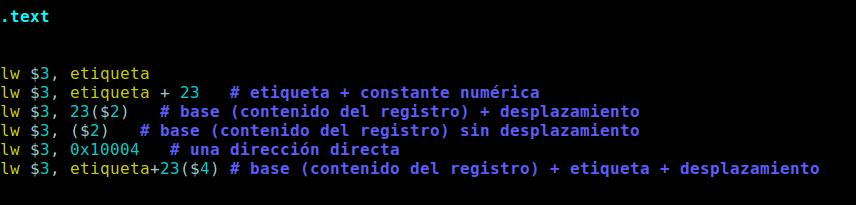
\includegraphics[scale=0.4]{images/formatos.jpg} 

%\begin{verbatim}
%lw $3, etiqueta
%lw $3, etiqueta+23   # etiqueta + constante numérica
%lw $3, 23($2)   # base (registro) + desplazamiento
%lw $3, ($2)   # base (registro) sin desplazamiento
%lw $3, 0x10004   # una dirección directa
%lw $3, 0x10004   # una dirección directa
%lw $3, etiqueta+23(\$5)  # base (registro) + etiqueta + constante numérica
%\end{verbatim}

\end{itemize}
\end{frame}


\begin{frame}
\frametitle{Programación de la máquina: lenguaje ensamblador MIPS}
        \begin{center}
        \textbf{Conjunto básico de instrucciones MIPS}
        \end{center}
\begin{tabular}{cl}

\begin{tabular}{c}
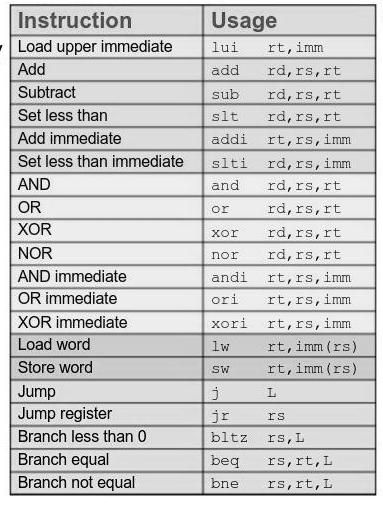
\includegraphics[height=5cm, width=4cm]{images/instrucciones-mips.jpg}

\end{tabular}
& \begin{tabular}{l}
\parbox{0.5\linewidth}{

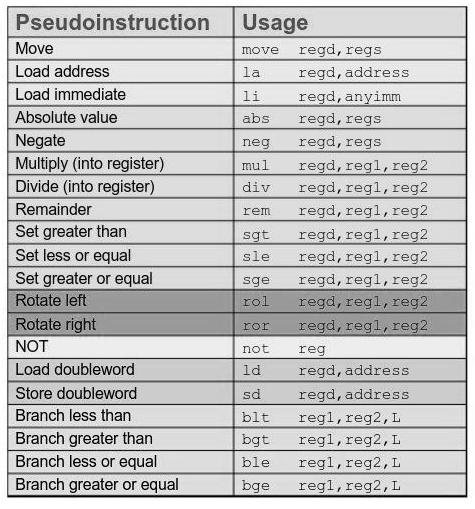
\includegraphics[height=5.2cm, width=4cm]{images/pseudoinstrucciones-mips2.jpg}
}
\end{tabular} \\

\end{tabular}
\end{frame}


\begin{frame}
\frametitle{Formato de  instrucciones en MIPS}
	\textbf{3 Formatos (fácil decodificación en hardware)}
	\begin{center}
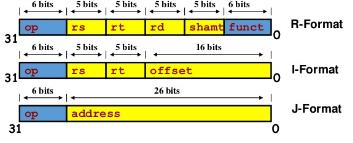
\includegraphics[scale=0.5]{images/formato.jpg} 
	\end{center}
\end{frame}


\begin{frame}
\frametitle{Formato de instrucciones en MIPS}
	\textbf{Un ejemplo completo de traducción al lenguaje de la máquina}
	\begin{center}
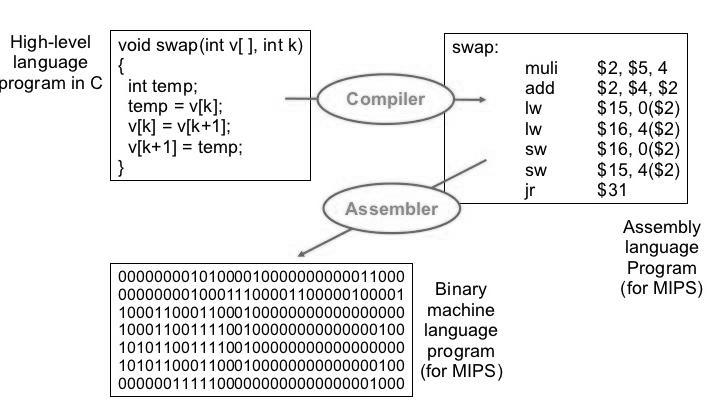
\includegraphics[scale=0.4]{images/below2.jpg} 
	\end{center}
\end{frame}





\begin{frame}
\frametitle{Tipos de Instrucciones}
\begin{center}\textbf{Tipos Principales de Instrucciones}\end{center}
\begin{itemize}
\item Aritméticas y Lógicas
\begin{itemize}
\item Enteros
\item Punto Flotante
\end{itemize}
\item Instrucciones de transferencia de datos (memoria)
\begin{itemize}
\item Carga y Almacenamiento
\end{itemize}
\item Flujo de control
\begin{itemize}
\item Salto
\item Bifurcación condicional
\item Llamado y Retorno
\end{itemize}
\end{itemize}
\end{frame}



\begin{frame}[fragile]
\frametitle{Tipos de Instrucciones}
\begin{center}\textbf{Instrucciones aritméticas en MIPS}\end{center}
\begin{itemize}
\item Las instrucciones aritméticas y lógicas más comunes tienen 3 operandos
\item El orden de los operandos es fijo (el destino primero)
\item Ejemplo:
\end{itemize}

\begin{verbatim}

  Código C:        a = b + c;

  Código MIPS:     add $s0, $s1, $s2

(el compilador asocia a $s0, $s1 y $s2 a las variables a, b y c)

\end{verbatim}

\end{frame}



\begin{frame}[fragile]
\frametitle{Tipos de Instrucciones}
\begin{center}\textbf{Instrucciones aritméticas en MIPS}\end{center}

\begin{verbatim}

  Código C:        a = b + c + d;
                   e = f - a;

  Código MIPS:     add $t0, $s1, $s2
                   add $s0, $t0, $s3
                   sub $s4, $s5, $s0
\end{verbatim}
\begin{itemize}
\item Los operandos deben estar en registros, y existen sólo 32
\item Principio de diseño: Más pequeño es más rápido. Porqué? (viaje de las señales)
\end{itemize}
\end{frame}





\begin{frame}
\frametitle{Tipos de instrucciones en MIPS}
\begin{center}\textbf{Registros vs. Memoria}\end{center}

\begin{itemize}
\item Los operandos deben estar en registros, y existen sólo 32
\item El compilador asocia variables a registros
\item ¿Qué sucede con un programa con un montón de variables?
\end{itemize}
\begin{center}
\begin{figure}
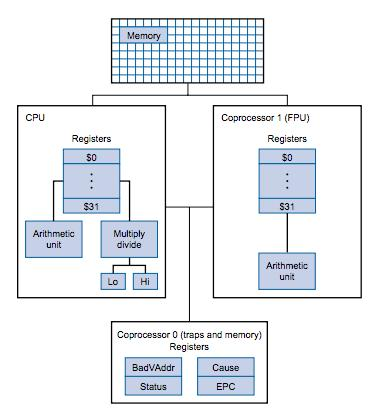
\includegraphics[scale=0.4]{images/organizacion-mips.jpg} 
\end{figure}
\end{center}
\end{frame}


\begin{frame}
\frametitle{Representación de datos a nivel máquina}
\textbf{Organización de la Memoria principal en MIPS}
\begin{itemize}
	\item $2^{32}$ bytes, con direcciones 0, 1, 2 ... 
	\item $2^{30}$ 4-bytes palabras, con direcciones 0, 4, 8 ... 
	\item Las direcciones de las palabras deben ser múltiplos de 4
\end{itemize}
	\begin{center}
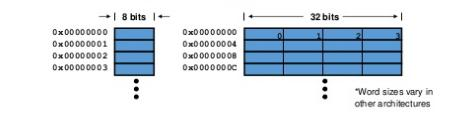
\includegraphics[scale=0.5]{images/memoria-mips.jpg} 
	\end{center}
\end{frame}


\begin{frame}[fragile]
\frametitle{Tipos de Instrucciones}
\begin{center}\textbf{Registros vs. Memoria}\end{center}

\begin{itemize}
\item Los operandos deben estar en registros, y existen sólo 32
\item El compilador asocia variables a registros
\item ¿Qué sucede con un programa con un montón de variables?
\end{itemize}
\end{frame}



\begin{frame}[fragile]
\frametitle{Tipos de Instrucciones}
\begin{center}\textbf{Asignación de Registros}\end{center}

\begin{itemize}
\item El compilador intenta asociar tantas variables a registros como sea posible
\item Algunas variables no pueden ser alocadas
\begin{itemize}
\item grandes arreglos (vectores)
\item variables accedidas con diferentes punteros
\item variables alocadas dinamicamente
\begin{itemize}
\item heap
\item stack
\end{itemize}
\end{itemize}
\item El compilador podría quedarse sin registros : \textbf{spilling}
\end{itemize}
\end{frame}



\begin{frame}[fragile]
\frametitle{Tipos de Instrucciones}
\begin{center}\textbf{Instrucciones de transferencia de datos}\end{center}

\begin{itemize}
\item Instrucciones de \textbf{Carga} y \textbf{Almacenamiento}
\item Ejemplo:
\end{itemize}
\begin{verbatim}

  Código C:        a[8] = h + a[8];

  Código MIPS:     lw  $t0, 32($s3)
                   add $t0, $s2, $t0
                   sw  $t0, 32($s3)
\end{verbatim}
\begin{itemize}
\item Las operaciones de carga y almacenamiento no tienen operandos destino (registro)
\item Recuerde: las operaciones aritméticas y lógicas operan sobre registros, no sobre elementos en la memoria!
\end{itemize}
\end{frame}




\begin{frame}
\frametitle{Formato de instrucciones en MIPS}
\begin{center}\textbf{Un ejemplo completo de traducción de C al lenguaje de la máquina}\end{center}
\begin{itemize}
\item ¿Puede interpretar la asignación de variables y el por qué del código en lenguaje ensamblador?
\end{itemize}
	\begin{center}
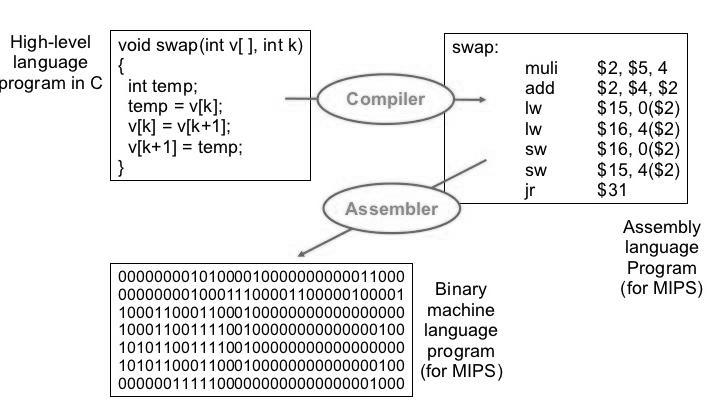
\includegraphics[scale=0.4]{images/below2.jpg} 
	\end{center}
\end{frame}




\begin{frame}[fragile]
\frametitle{Tipos de Instrucciones}
\begin{center}\textbf{Repaso}\end{center}

\begin{itemize}
\item MIPS
\begin{itemize}
\item Cargamos palabras (words) pero utilizamos direccionamiento del primer byte
\item Las instrucciones aritméticas y lógicas operan unicamente con registros
\end{itemize}
\end{itemize}
\begin{verbatim}

  Instrucción            Significado

  add $s1, $s2, $s3      $s1 = $s2 + $s3
  sub $s1, $s2, $s3      $s1 = $s2 - $s3
  lw $s1, 100($s2)       $s1 = MEMORIA[$s2+100]
  sw $s1, 100($s2)       MEMORIA[$s2+100] = $s1
\end{verbatim}
\end{frame}


\begin{frame}[fragile]
\frametitle{Lenguaje Máquina}
\begin{center}\textbf{Formato de Instrucciones en MIPS}\end{center}
\begin{itemize}
\item Las instruccciones, como los registros y la palabra, son de 32-bits
\begin{itemize}
\item Los registros están numerados en el código máquina: del 0 al 31
\end{itemize}
\end{itemize}
	\begin{center}
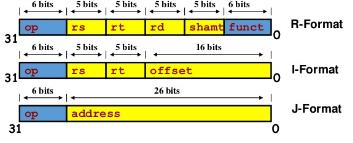
\includegraphics[scale=0.7]{images/formato.jpg} 
	\end{center}
\end{frame}



\begin{frame}[fragile]
\frametitle{Tipos de Instrucciones}
\begin{center}\textbf{Instrucciones de transferencia de Control}\end{center}

\begin{itemize}
\item Instrucciones para realizar decisiones
\begin{itemize}
\item Alterar el flujo de control de ejecución
\item y por lo tanto, cambiar la "próxima" instrucción a ser ejecutada
\end{itemize}
\item Instrucciones de bifurcación condicional en MIPS
\begin{verbatim}
                bne $t0, $t1, label
                beq $t0, $t1, label
\end{verbatim}
\item Ejemplo:
\begin{verbatim}
   Código en C:      if (i == j)  h = i + j;

   Código en MIPS:         bne $s0, $s1, label
                           add $s3, $s0, $s1
                     label: ...
\end{verbatim}
\end{itemize}
\end{frame}




\begin{frame}[fragile]
\frametitle{Tipos de Instrucciones}
\begin{center}\textbf{Instrucciones de transferencia de Control}\end{center}

\begin{itemize}
\item Instrucciones de salto incondicional
\begin{itemize}
\item j  label
\end{itemize}
\item Ejemplo:
\begin{verbatim}
   Código en C:      if (i != j)  
                           h = i + j;
                     else
                           h = i - j;


   Código en MIPS:         beq $s4, $s5, lab1
                           add $s3, $s4, $s5
                           j lab2
                     lab1: sub $s3, $s4, $s5
                     lab2:
\end{verbatim}
\end{itemize}
\end{frame}




\begin{frame}[fragile]
\frametitle{Tipos de Instrucciones}
\begin{center}\textbf{Repaso}\end{center}

\footnotesize
\begin{verbatim}

Instrucción            Significado

add $s1, $s2, $s3      $s1 = $s2 + $s3
sub $s1, $s2, $s3      $s1 = $s2 - $s3
lw $s1, 100($s2)       $s1 = MEMORIA[$s2+100]
sw $s1, 100($s2)       MEMORIA[$s2+100] = $s1
bne $s4, $s5, Etiq     Próx. instr. está en Etiq si $s4 es distinto a $s5
beq $s4, $s5, Etiq     Próx. instr. está en Etiq si $s4 es igual a $s5
j Etiqueta             Próx. instr. está en Etiqueta

\end{verbatim}
\end{frame}


\begin{frame}[fragile]
\frametitle{Tipos de Instrucciones}
\begin{center}\textbf{Instrucciones de transferencia de Control}\end{center}

\begin{itemize}
\item Salto condicional: bne, beq
\item ¿Qué sucede con saltar si es menor qué?
\item Nueva instrucción:
\begin{verbatim}
   slt $t0, $s1, $s2

Significado:      if $s1 < $s2 then
                      $t0 = 1
                  else
                      $t0 = 0
\end{verbatim}
\item Puede ser utilizada para construir \begin{verbatim}"blt $s1, $s2, Etiqueta"\end{verbatim}
\begin{itemize}
\item Se pueden construir estructuras de control de ejecución generales
\end{itemize}
\item El ensamblador necesita utilizar un registro \textit{temporal}
\begin{itemize}
\item Convención de uso de registros
\end{itemize}
\end{itemize}
\end{frame}


\begin{frame}
\frametitle{Modelo de programación MIPS}
        \begin{center}
        \textbf{Convención de uso de registros en MIPS}
 \\~\\

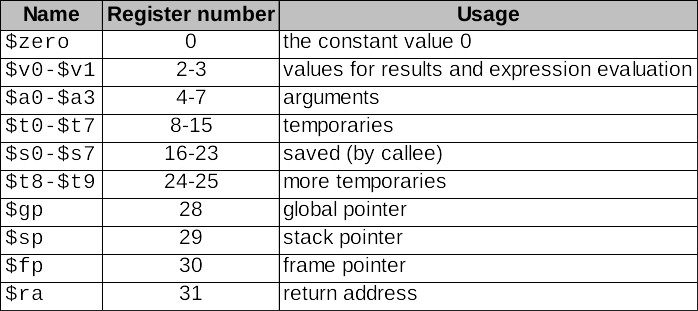
\includegraphics[scale=0.3]{images/convencion.jpg}

        \end{center}
\end{frame}


\begin{frame}[fragile]
\frametitle{Modelo de programación MIPS}
\begin{center}\textbf{Constantes}\end{center}

\begin{itemize}
\item Pequeñas constantes son utilizadas muy frecuentemente (50 por ciento de los operandos son constantes)
\begin{verbatim}
Ejemplo:   a = a + 5;
           b = b + 1 ;
           c = c * 2 + 1;
\end{verbatim}
\item ¿Soluciones? 
\begin{itemize}
\item Poner las constantes típicas (1, 2, 10) en memoria y cargarlas
\item Crear registros cableados en hardware con un valor (hard-wired). Como el registro zero
\item o .....
\end{itemize}
\item Colocar las constantes como parte de las Instrucciones (MIPS)
\begin{verbatim}
Ejemplo:   addi $29, $29 + 5
           addi $8, $8, 1
           andi $29, $29, 6
           ori $9, $9, 4
\end{verbatim}
\end{itemize}
\end{frame}




\begin{frame}[fragile]
\frametitle{Modelo de programación MIPS}
\begin{center}\textbf{¿Qué sucede con grandes Constantes?}\end{center}

\begin{itemize}
\item Las instrucciones son de 32-bits, por lo que no es posible colocar una constantes de 32-bits dentro de la instrucción.
\item Solución: para cargar una constante de 32-bit en un registro se utilizan dos instrucciones
\begin{verbatim}
Ejemplo:   lui $t0, 0xAAAA
           ori $t0, 0xAAAA
\end{verbatim}
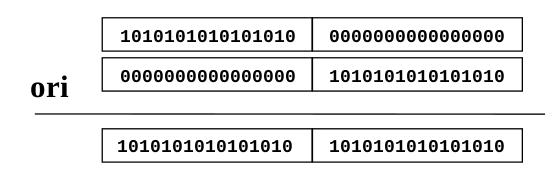
\includegraphics[scale=0.4]{images/ori.jpg}
\end{itemize}
\end{frame}







\begin{frame}
\frametitle{Programación de la máquina: lenguaje ensamblador MIPS}
        \begin{center}
        \textbf{Conjunto básico de instrucciones MIPS}
        \end{center}
\begin{tabular}{cl}

\begin{tabular}{c}
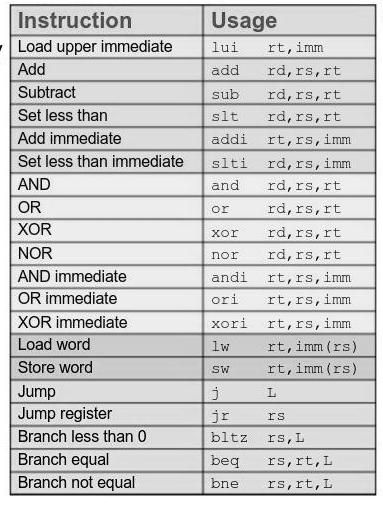
\includegraphics[height=5cm, width=4cm]{images/instrucciones-mips.jpg}

\end{tabular}
& \begin{tabular}{l}
\parbox{0.5\linewidth}{

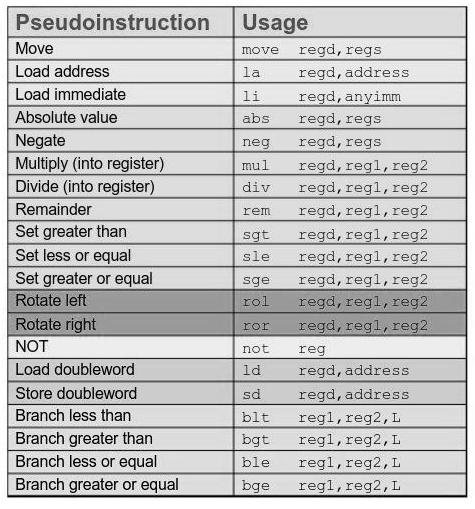
\includegraphics[height=5.2cm, width=4cm]{images/pseudoinstrucciones-mips2.jpg}
}
\end{tabular} \\

\end{tabular}
\end{frame}


\begin{frame}[fragile]
\frametitle{Modelo de programación MIPS}
\begin{center}\textbf{Resumen de la arquitectura MIPS}\end{center}
\begin{itemize}
\item Instrucciones sencillas de 32-bits de ancho
\item Muy estructurado, no hay necesidad de grandes variaciones
\item Confía en el compilador para ganar performance
\item Hay que ayudar al compilador cuando sea necesario
\item Únicamente 3 formatos de instrucciones
	\begin{center}
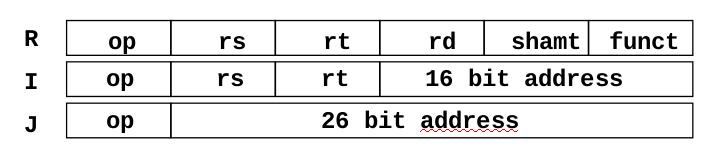
\includegraphics[scale=0.3]{images/formato2.jpg} 
	\end{center}
\item ¿Cómo programar mejor? (cantidad de variables, constantes)
\end{itemize}
\end{frame}


\subsection{Modos de direccionamiento}

\begin{frame}[fragile]
\frametitle{Modos de direccionamiento}
\begin{itemize}
\item Los modos de direccionamiento son las diferentes formas de especificar un operando dentro de una instrucción (a nivel código máquina).
\item \textbf{NO CONFUNDIR modos de direccionamiento con los formatos de direccionamiento} permitidos al programar en lenguaje ensamblador
\item La literatura los clasifica en: Inmediato, Directo, Indirecto, Registro, Indirecto por registro, Basado-indexado (base+desplazamiento), Pila.
\end{itemize}
\end{frame}


\begin{frame}{Modos de direccionamiento}
\begin{center}\textbf{Inmediato (constante)}\end{center}
El operando se encuentra en la instrucción.

Ejemplo: \texttt{addi \$s0, \$s1, 87} 

	\begin{center}
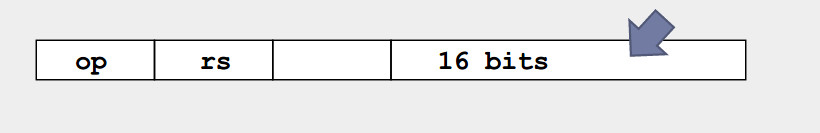
\includegraphics[scale=0.3]{images/dir-inmediato.jpg} 
	\end{center}
\end{frame}


\begin{frame}{Modos de direccionamiento}
\begin{center}\textbf{Registro}\end{center}

\begin{itemize}
\item El operando se encuentra en un registro.
\item La instrucción máquina indica el registro.
\item Ejemplo: \texttt{add \$s0, \$s1, \$s4} 

\end{itemize}

	\begin{center}
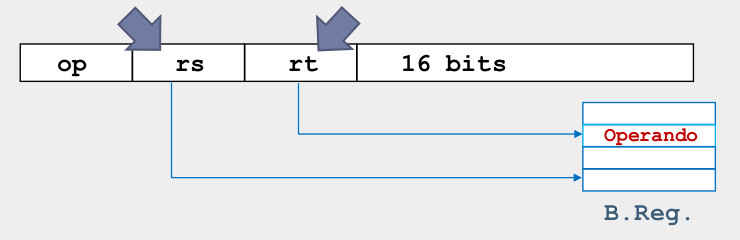
\includegraphics[scale=0.3]{images/dir-registro.jpg} 
	\end{center}
\end{frame}


\begin{frame}{Modos de direccionamiento}
\begin{center}\textbf{Indirecto}\end{center}

\begin{itemize}
\item El operando se encuentra en memoria.
\item La instrucción máquina indica una dirección de memoria, que apunta a la dirección de memoria (dirección efectiva) del operando.
\item Ejemplo: No existe en MIPS
\item Es útil en lenguajes de alto nivel como C para los arreglos y punteros.

\end{itemize}

	\begin{center}
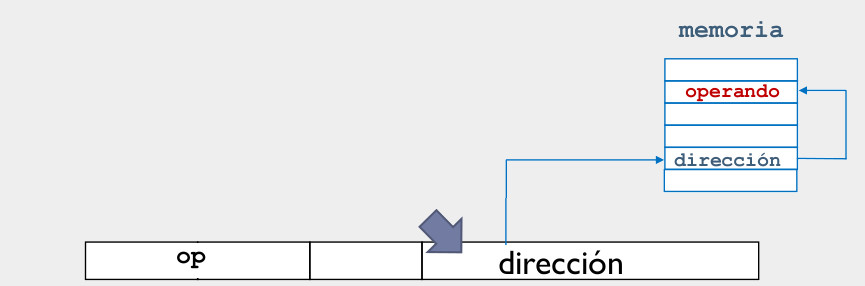
\includegraphics[scale=0.3]{images/dir-indirecto.jpg} 
	\end{center}
\end{frame}


\begin{frame}{Modos de direccionamiento}
\begin{center}\textbf{Indirecto por registro}\end{center}

\begin{itemize}
\item El operando se encuentra en memoria.
\item La instrucción máquina indica un registro, que apunta a (contiene) la dirección de memoria (dirección efectiva) del operando.
\item Ejemplo: En MIPS existe, pero lleva siempre un desplazamiento que podría ser cero (base + desplazamiento). \texttt{lw \$s0, 0(\$s1)}
\item Es útil en lenguajes de alto nivel como C para los arreglos y punteros.

\end{itemize}

	\begin{center}
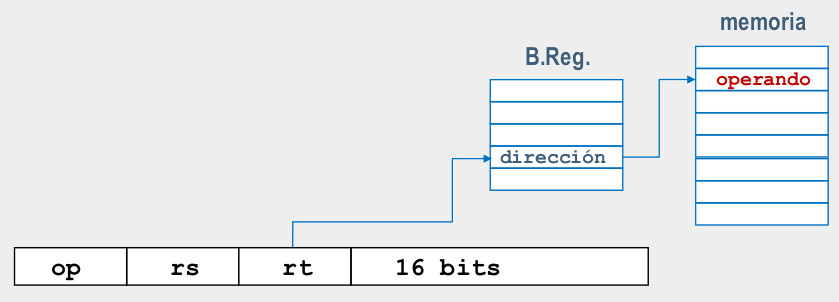
\includegraphics[scale=0.3]{images/dir-indirecto-por-registro.jpg} 
	\end{center}
\end{frame}


\begin{frame}{Modos de direccionamiento}
\begin{center}\textbf{Base mas desplazamiento (indexado)}\end{center}

\begin{itemize}
\item El operando se encuentra en memoria.
\item La instrucción máquina indica un registro más una constante. Sumando el contenido del registro, mas la constante, se logra la dirección efectiva.
\item Ejemplo: \texttt{lw \$s0, 33(\$s1)}
\item Es útil en lenguajes de alto nivel como C para estructuras de datos. El compilador puede colocar la dirección base de la estructura en el registro, y generar los desplazamientos a cada miembro, ya que son de distancia fija.

\end{itemize}

	\begin{center}
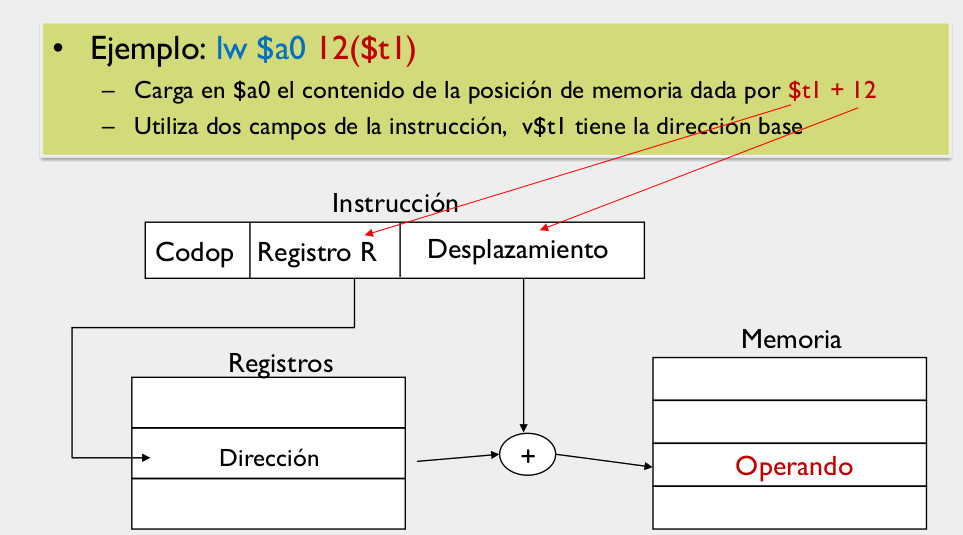
\includegraphics[scale=0.18]{images/dir-base-desplazamiento.jpg} 
	\end{center}
\end{frame}


\begin{frame}{Modos de direccionamiento}
\begin{center}\textbf{Basado Indexado}\end{center}

\begin{itemize}
\item El operando se encuentra en memoria.
\item La instrucción máquina indica dos registros. Se suman los contenidos de ambos registros, y se logra la dirección efectiva del operando.
\item Ejemplo: En MIPS no existe. Podría ser: \\ \texttt{load  A, B, C  \# cargar en A el operando en la dirección efectiva B+C}
\item Es útil en lenguajes de alto nivel como C para arreglos de estructuras.

\end{itemize}

\end{frame}

\begin{frame}{Modos de direccionamiento}
\begin{center}\textbf{Pila}\end{center}

\begin{itemize}
\item El operando se encuentra en la pila.
\item La instrucción máquina SÓLO indica la operación (por ejemplo: add). Los operandos son implícitos (el tope de la pila).
\item Ejemplo: En MIPS no existe. 
\item En una arquitectura de pila la instrucción podría ser \textbf{add}, y la CPU desapila dos elementos del tope de la pila, los suma, y coloca el resultado en el tope de la pila.
\item Es útil en arquitecturas donde las instrucciones deban ocupar poco espacio.

\end{itemize}

\end{frame}




\begin{frame}[fragile]
\frametitle{Modos de direccionamiento}
\begin{center}\textbf{Modos de direccionamiento en MIPS}\end{center}
	\begin{center}
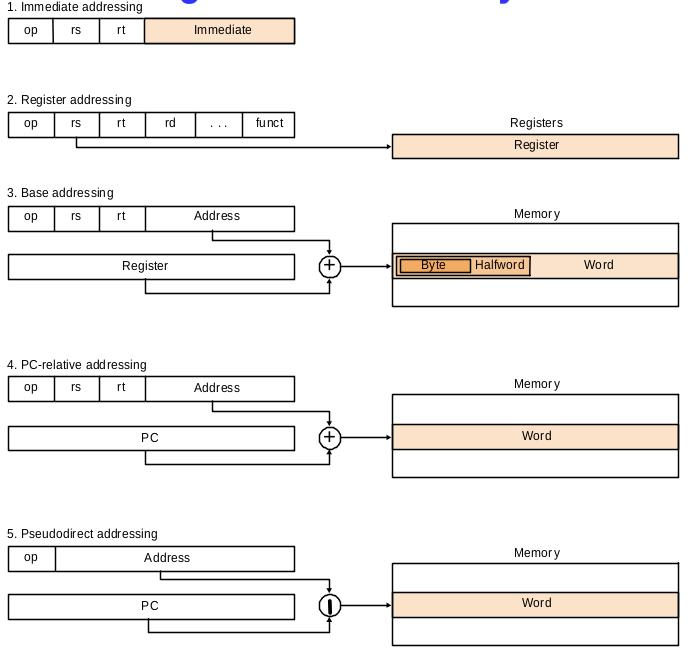
\includegraphics[scale=0.3]{images/modos-de-direccionamiento.jpg} 
	\end{center}
\end{frame}



\subsection{lenguaje ensamblador vs lenguaje máquina}

\begin{frame}[fragile]
\frametitle{Modelo de programación MIPS}
\begin{center}\textbf{Lenguaje Ensamblador vs. Lenguaje Máquina?}\end{center}

\begin{itemize}
\item El lenguaje ensamblador provee una representación simbólica conveniente
\begin{itemize}
\item Es mucho más sencillo que programar escribiendo números
\item Por ejemplo: el destino de una operación va primero
\end{itemize}
\item El lenguaje máquina es la verdadera realidad
\begin{itemize}
\item Por ejemplo: el destino ya no es lo primero que aparece en una operación va primero
\end{itemize}
\item El lenguaje ensamblador puede proveer \textbf{pseudoinstrucciones}
\begin{itemize}
\item Por ejemplo: \begin{verbatim}move $t0, $t1\end{verbatim}
\item sería implementadao utilizando:  \begin{verbatim}add $t0, $t1, $zero\end{verbatim}
\end{itemize}
\item Cuando se debe considerar la performance se deben contar las instrucciones reales
\end{itemize}
\end{frame}



\begin{frame}
 \frametitle{Bibliografía}
Libros
\begin{itemize}
\item Andrew S. Tanenbaum (2000), ORGANIZACIÓN DE COMPUTADORAS un enfoque estructurado, Editorial Prentice Hall. (10 copias en biblioteca)
\item David. Patterson John L. Hennessy (1995), ORGANIZACIÓN Y DISEÑO DE COMPUTADORES La interfaz hardware/software, McGraw-Hill (8 copias en biblioteca).
\end{itemize}
Contenido electrónico
\begin{itemize}
	\item \textbf{x86 assembly basis} Una introducción al lenguaje ensamblador x86. Disponible en PEDCO en formato PDF.
		\url{https://www.nayuki.io/page/a-fundamental-introduction-to-x86-assembly-programming}
\item Apuntes elaborados por la cátedra, disponibles en PEDCO para impresión (pdf) o lectura online (html)
\item Secciones de libros aptas para publicacion
\end{itemize}
\end{frame}

\end{footnotesize}

\end{document}
